\documentclass[a4paper,notitlepage]{article}
\usepackage[utf8]{inputenc} %Make sure all UTF8 characters work in the document
\usepackage{listings} %Add code sections
\usepackage{color}
\usepackage[yyyymmdd]{datetime}
\usepackage{graphicx}
\usepackage{titling}
\usepackage{titlesec}
\usepackage{listliketab}
\usepackage{textcomp}
\usepackage[hyphens]{url}
\usepackage[bottom]{footmisc}
\definecolor{listinggray}{gray}{0.9}
\definecolor{lbcolor}{rgb}{0.9,0.9,0.9}
\usepackage{geometry}
\geometry{margin=3cm}
\usepackage{parskip} 
\renewcommand{\dateseparator}{--}
\renewcommand{\arraystretch}{1.3}
\titlespacing*\section{0pt}{10pt plus 4pt minus 2pt}{0pt plus 2pt minus 2pt}
\titlespacing*\subsection{0pt}{10pt plus 4pt minus 2pt}{0pt plus 2pt minus 2pt}
\pretitle{%
\begin{center}
	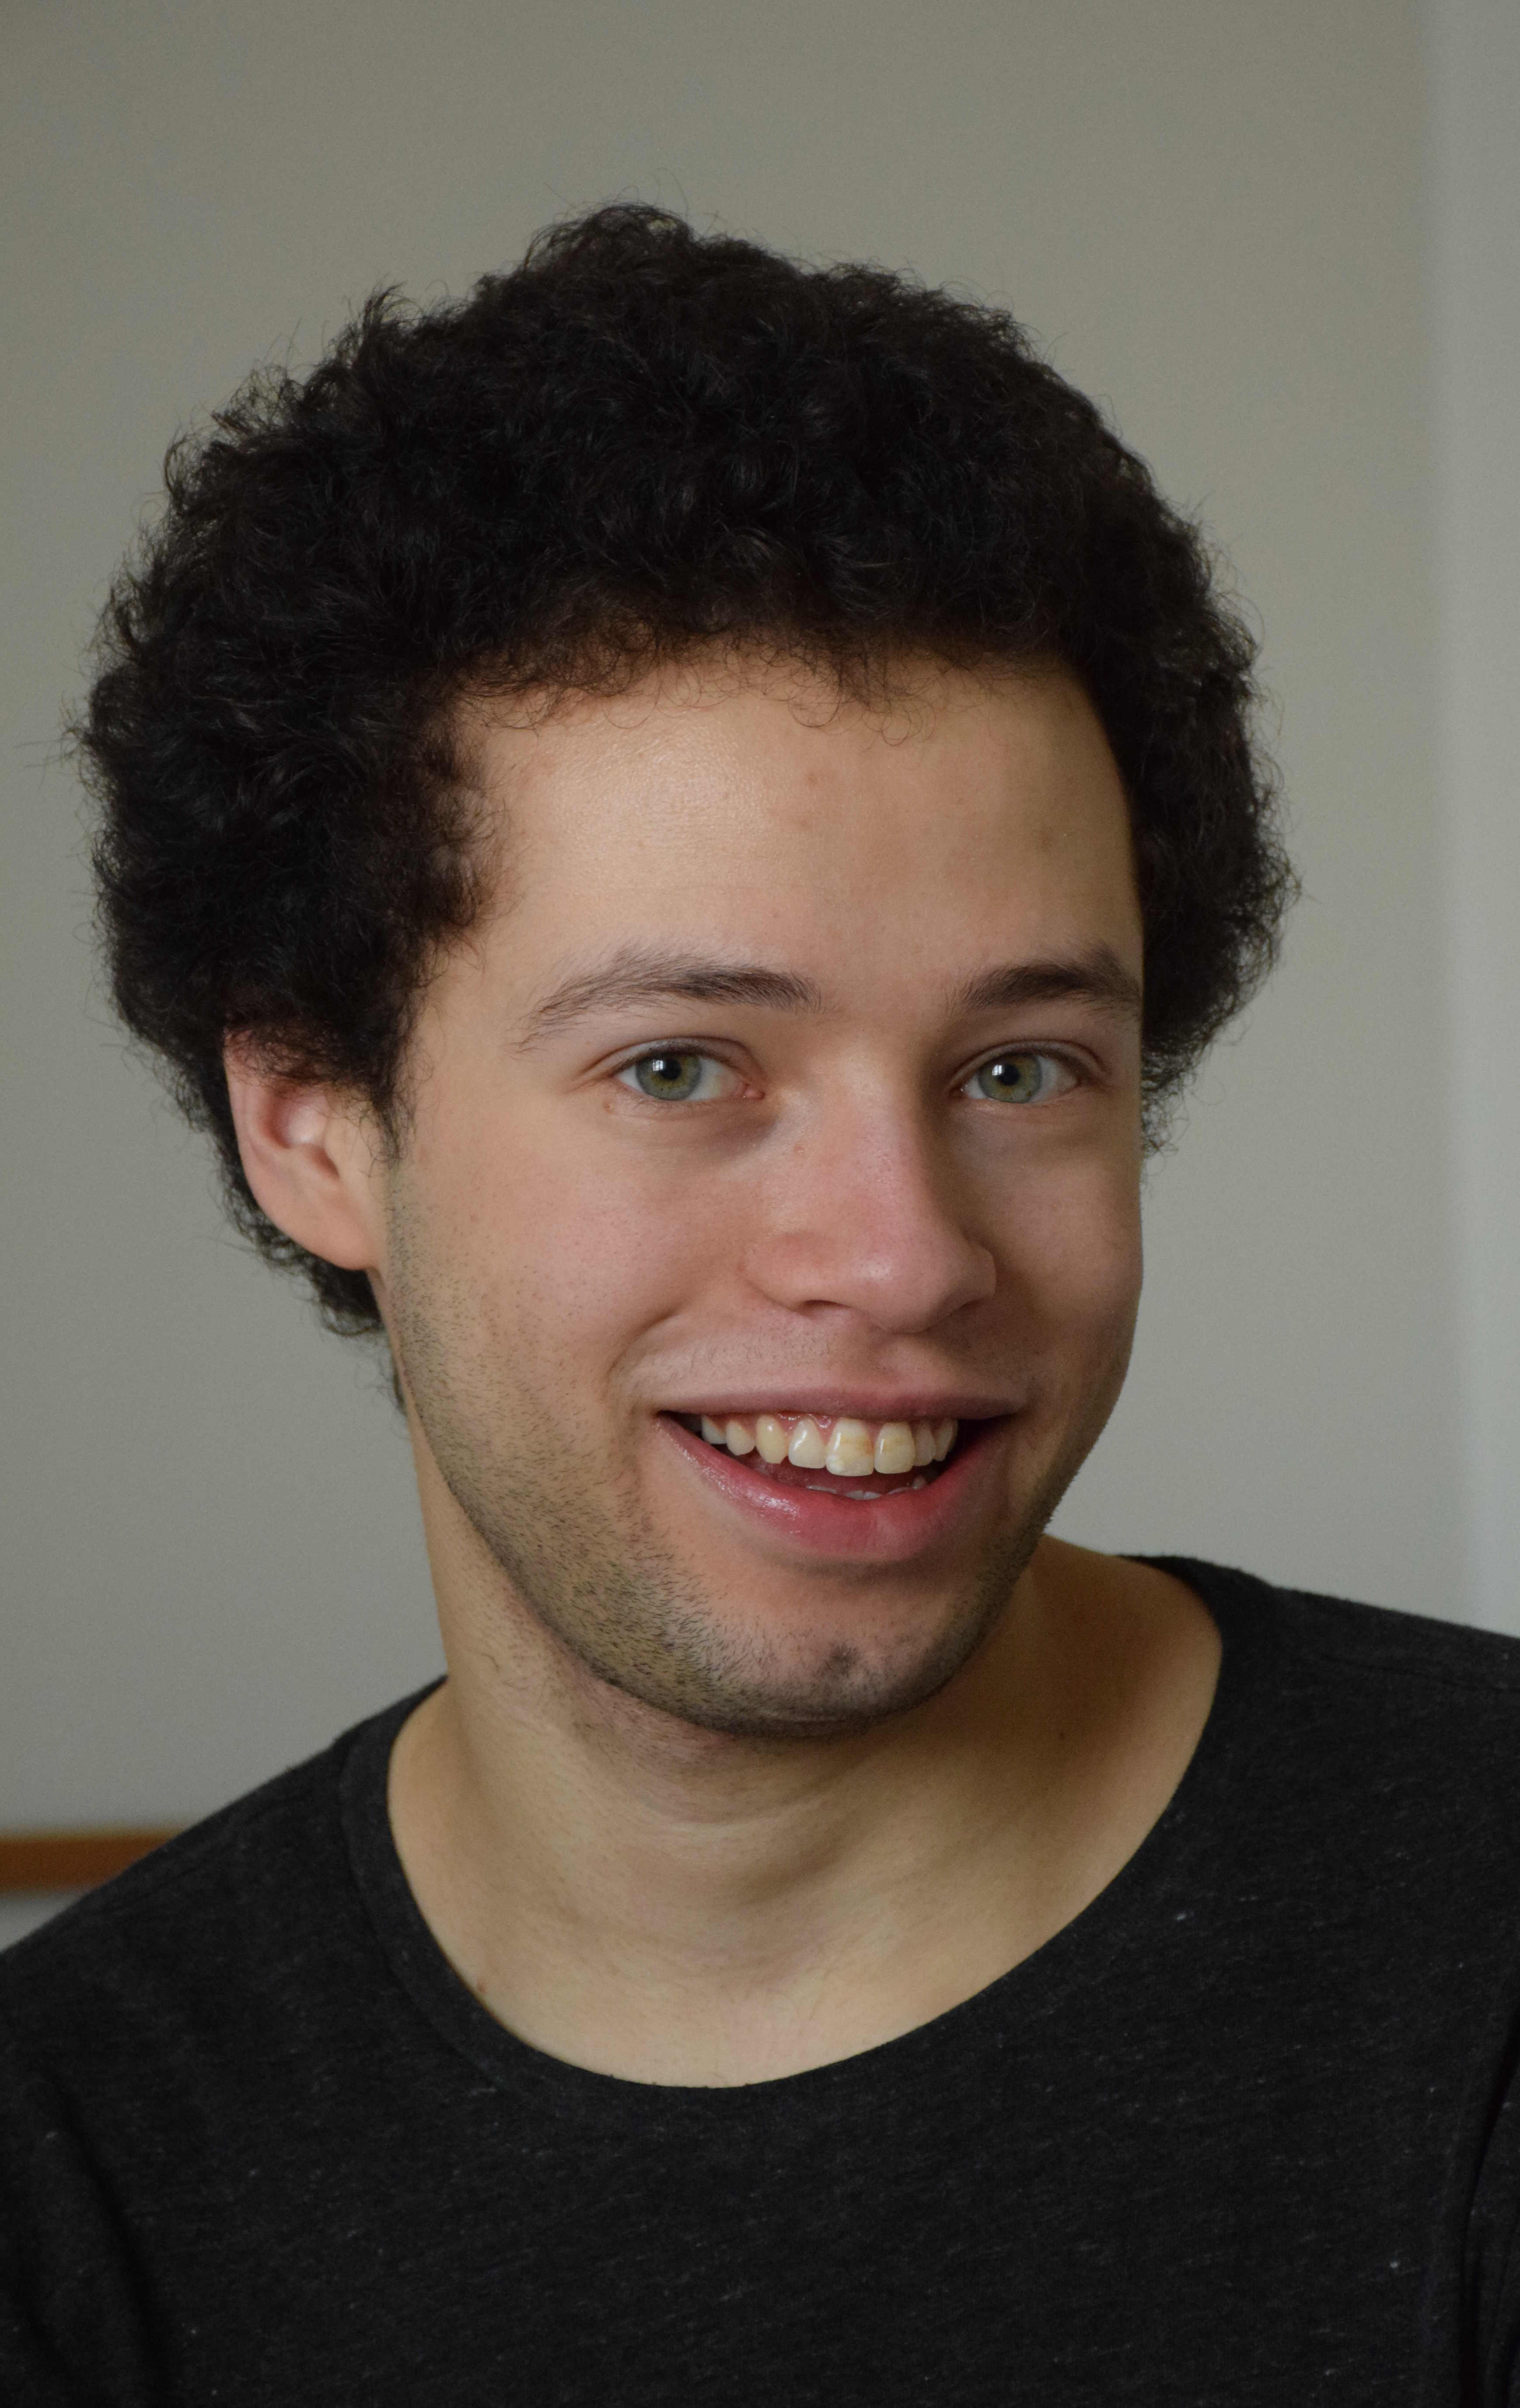
\includegraphics[width=4cm]{bild.jpeg}\\[\bigskipamount]
	% TODO hitta en bättre bild
}
\posttitle{\end{center}}
\title{
\huge{CV - Malcolm Vigren}\vspace{-3ex}}
\date{\today}
\begin{document}
	\maketitle
\underline{Malcolm} John Shubi Vigren, 19950127-0970

Batterigatan 9

587 50 Linköping

E-post: \underline{malcolm.w@me.com}

Mobil: 072-534 16 81	

\section*{Arbetslivserfarenhet}
\noindent\begin{tabular}{@{}l p{13cm}}

\textbf{2016} & Sommarjobb på Autoliv i Linköping. Utvecklade verktyg för
    utförande av regressionstester i Python och C\#.\\

\textbf{2015 - 2016:} & Butiksarbetare på ICA Supermarket Eneby i Norrköping, med
arbetsuppgifter som kassör, spelombudsbiträde och postombudsbiträde, vid sidan
av universitetsstudier. \\

\textbf{2013:} & Skapade en animerad film åt SundaHus för en mässa.
\\

\textbf{2012 - 2015:} & Butiksarbetare på Hemköp Ljungsbrohallen,
med arbetsuppgifter
som kassör,
spelombudsbiträde, postombudsbiträde, ansvarig för ändring av priser med mera.
\\

\textbf{2010:} & PRAO i fem dagar på Hemköp Ljungsbrohallen under
höstterminen. \\

\textbf{2010:} & PRAO i tre dagar på ABB Service-verkstaden i
Norrköping på vårterminen. \\

\textbf{2010 - 2013:} & Städning av judolokalen i Linköping en gång
i veckan. \\

\textbf{2008 - 2012:} & Inmatning av produktinformation i SundaHus Miljödatabas under
skolloven.	\\

	\end{tabular}

\section*{Utbildning}
\noindent\begin{tabular}{@{}l p{11cm}}
	\textbf{Högskola:} & \textit{Linköpings Universitet} - Civilingenjör i
	datateknik 300hp - Pågående, påbörjad HT2014 \\

	\textbf{Gymnasieskola:} & \textit{Berzeliusskolan} - Teknikvetenskap -
	Avslutad, examen 2014 \\

	\textbf{Grundskola:} & \textit{Internationella Engelska Skolan i Linköping},
	årskurs 6-9 \\

	\textbf{Grundskola:} & \textit{Brunnbyskolan}, årskurs 1-5 \\
	\end{tabular}

%\subsection*{Avslutade universitetskurser}
%\noindent\begin{tabular}{@{}l l l l}
%	\textbf{TDDD84} & \textit{Ingenjörsprofessionalism, del 3} & 1 hp & Betyg 5 \\
%	\textbf{TATA24} & \textit{Linjär algebra} & 8 hp & Betyg 5 \\
%	\textbf{TSEA82} & \textit{Datorteknik} & 4 hp & Betyg G \\
%	\textbf{TDDD78} & \textit{Objektorienterad programmering och Java} & 6 hp & Betyg 5 \\
%	\textbf{TDDD94} & \textit{Ingenjörsprofessionalism, del 4} & 1 hp & Betyg 5 \\
%	\textbf{TGTU50} & \textit{Industrikunskap} & 1.5 hp & Betyg D (deltagit) \\
%	\textbf{TSEA22} & \textit{Digitalteknik} & 6 hp & Betyg 4 \\
%	\textbf{TSTE21} & \textit{Elektronik} & 5 hp & Betyg G \\
%	\textbf{TATA42} & \textit{Envariabelanalys 2} & 6 hp & Betyg 3 \\
%	\textbf{TATA41} & \textit{Envariabelanalys 1} & 6 hp & Betyg 4 \\
%	\textbf{TATA79} & \textit{Inledande matematisk analys} & 6 hp & Betyg 3 \\
%	\textbf{TDDD70} & \textit{Ingenjörsprofessionalism del 1} & 1 hp & Betyg 5 \\ 
%	\textbf{TDDD63} & \textit{Perspektiv på datavetenskap} & 7 hp & Betyg G \\
%	\textbf{TDDD73} & \textit{Funktionell och imperativ programmering i Python} & 4 hp &
%	Betyg 4 \\
%	\textbf{TATA65} & \textit{Diskret Matematik} & 4 hp & Betyg 4 \\
%	\textbf{TDDC66} & \textit{Datorsystem och programmering} & 4 hp & Betyg G \\
%	\end{tabular}
%\subsection*{Kurser avslutade till VT2016}
%\noindent\begin{tabular}{@{}l l l}
%	\textbf{TDDD86} & \textit{Datastrukturer, algoritmer och
%programmeringsparadigm} & 11 hp \\
%	\textbf{TFYY68} & \textit{Mekanik} & 6 hp \\
%	\textbf{TATA76} & \textit{Flervariabelanalys} & 4 hp \\
%	\textbf{TSEA83} & \textit{Datorkonstruktion} & 8 hp \\
%	\textbf{TDDB68} & \textit{Processprogrammering och operativsystem} & 6 hp \\
%	\textbf{TDDD98} & \textit{Ingenjörsprofessionalism del 6} & 1 hp \\
%	\textbf{TAMS27} & \textit{Matematisk statistik} & 6 hp \\
%	\textbf{TSRT04} & \textit{Introduktionskurs i Matlab} & 2 hp \\
%	\textbf{TFYA86} & \textit{Fysik} & 6 hp \\
%	\end{tabular}
\section*{Programmeringskunskaper}
Goda kunskaper inom C, C\#, C++, Java, Python, VHDL och assembler. Viss kunskap inom HTML,
JavaScript, bash-skript och Haskell. Goda kunskaper inom versionshanteringsverktyget Git
och texteditorn VIM, och viss kunskap inom simuleringsprogrammet ModelSim.
\section*{Språkkunskaper}
Flytande svenska och engelska i tal och skrift. Gymnasiekunskaper inom tyska
(Tyska steg 3).
\section*{Profil och intressen}
Jag är systematisk, noggrann och lättlärd. Jag är engagerad i mitt arbete och
försöker alltid att göra mitt bästa. Mina huvudintressen är vetenskap, teknik, matematik och datorer.

\section*{Övriga meriter}
Körkort (AM- samt B-behörighet).

Var med i vinnarlaget i en av tävlingarna under LiTHe Kods Jubileumshack den
12-13:e februari 2016, i vilken en algoritm för möblering och visualisering av 
ett rum skulle utvecklas över natten.

Erhöll 1000 kr ur Berzeliusskolans stipendiefond vid examen för mina höga
betyg.
\end{document}
